\documentclass[12pt,letterpaper]{article}
\usepackage{fullpage}
\usepackage[top=2cm, bottom=4.5cm, left=2cm, right=2cm]{geometry}
\usepackage{amsmath,amsthm,amsfonts,amssymb,amscd}
\usepackage{lastpage}
\usepackage{enumerate}
\usepackage{enumitem}
\usepackage{fancyhdr}
\usepackage{mathrsfs}
\usepackage{xcolor}
\usepackage{graphicx}
\graphicspath{{images/}}
\usepackage{subcaption}
\usepackage{amsmath}
\usepackage{listings}
\usepackage{hyperref}
\usepackage{float}
\usepackage{empheq}
\usepackage{blindtext}
\usepackage[makeroom]{cancel}
%\usepackage[framed,numbered,autolinebreaks,useliterate]{mcode}
% \documentclass{article}% or something else
\usepackage{pdfpages}
\usepackage{subfiles} % Best loaded last in preamble

\hypersetup{%
  colorlinks=true,
  linkcolor=blue,
  linkbordercolor={0 0 1}
}
 
\renewcommand\lstlistingname{Algorithm}
\renewcommand\lstlistlistingname{Algorithms}
\def\lstlistingautorefname{Alg.}

\lstdefinestyle{Python}{
    language        = Python,
    frame           = lines, 
    basicstyle      = \footnotesize,
    keywordstyle    = \color{blue},
    stringstyle     = \color{green},
    commentstyle    = \color{red}\ttfamily
}

\setlength{\parindent}{0.0in}
\setlength{\parskip}{0.05in}

% Edit these as appropriate
\newcommand\course{ME579}
\newcommand\hwnumber{HW 3}                  % <-- homework number
\newcommand\NetIDa{Colin Acton, Win Khoo, Rishi Jha}           % <-- NetID of person #1
\newcommand\duedate{}


% Common commands
\newcommand{\Laplace}[1]{\mathcal{L}\{#1\}}
\newcommand{\LaplaceInv}[1]{\mathcal{L}^{-1}\{#1\}}
\newcommand{\Z}[1]{\mathcal{Z}\{#1\}}
\newcommand{\ZInv}[1]{\mathcal{Z}^{-1}\{#1\}}
\newcommand\goesto{\rightarrow}
\newcommand\xvec{\textbf{x}}
\newcommand\dxvec{\dot{\textbf{x}}}
\newcommand\ddxvec{\ddot{\textbf{x}}}
\newcommand\tvec{\textbf{t}}
\newcommand\A{\textbf{A}}
\newcommand\B{\textbf{B}}
\newcommand\C{\textbf{C}}
\newcommand\D{\textbf{D}}
\newcommand\I{\textbf{I}}
\newcommand\T{\textbf{T}}
\newcommand\LambdaMat{\mathbf{\Lambda}}
\newcommand\Adj{\text{Adj}}
\newcommand\N{\textbf{N}}
\newcommand\J{\textbf{J}}
\newcommand\Q{\textbf{Q}}

\pagestyle{fancyplain}
\headheight 35pt
\lhead{\NetIDa}
\chead{\textbf{\Large Homework 3}}
\rhead{\course \\ \duedate}
\lfoot{}
\cfoot{}
\rfoot{\small\thepage}
\headsep 1.5em

\begin{document}

\section{Related Work}
\textbf{Briefly summarize some approaches that have been tried in the literature [1]. This does not have to be comprehensive but is intended to help you think of different strategies. Since training your models can be quite time-consuming. We encourage you to think through different approaches before settling on your final algorithm.}

The approaches to training the Tetris discussed in the literature [1] are categorized into four methods, namely hand-tuning, machine learning, optimizing, and the evolution way. Generally speaking, the final goal of all these approaches is to locate the optimal weights for the features that will maximize the total rewards (discussed under the reward section) which hopefully will clear as many lines as possible. A brief discussion of training methods is as the following in the same order mentioned above. The most straightforward way is to have one earn experience from playing the game Tetris and using one's mental judgment to assign the weights for the respective features. On the other hand, machine learning is one way when a set of data is provided for the training to figure out the optimal values of the feature's weights. Meanwhile, reinforcement learning could also be used to obtain the same objective. All in all, figuring out the optimal policy is the key to scoring the game instead of evaluating the value of the game state as value iteration is comparatively more costly than policy iteration which is unreal in practice. The optimal weights of the features can also be found through optimization techniques and evolution strategies to optimize the weights. Without doing excessive experiments and simply judging from the literature [1], the increasing number of used features does not necessarily guarantee better results in obtaining the weight's values. Instead, the design of features that can possibly capture and truly describe the ups and downsides of the actions and consequences of each implemented action. At last, literature 1 implemented the so-called covariance matrix adaptations a.k.a CMA which is an evolutionary approach and is similar to the cross-entropy method. Here, we started with using the Nelder-Mead and then the noisy cross-entropy method, and the details are discussed as follows.

\section{Cost Function}
\textbf{Describe what you used as a cost function and why.}

For our cost/value function we decided to use the weighted sum-of-features proposed by Boumaza et al [1]. Concretely, letting $\{f_i\}_{i=1}^{8}$ represent their feature functions (explained in more detail in the State Representation section), the value of a given state is as follows: $$V_w(s) = \sum_{i=1}^nw_if_i(s)$$
We found that this formulation had two distinct advantages in 1) simplifying the solution space and 2) adding interpretability as we developed the method. First off, the usage of feature functions allowed us to condense the large space of possible board states into a set of features we deemed important in determining the state of the game. In addition, unlike some more complex neural-network based architectures, it was fast and at each iteration of our weight-optimization algorithm we knew exactly why our model made the decisions it made.

\section{Rewards}
\textbf{Provide concrete definitions of your rewards and include some motivation for why you picked them.}

Just as most of us would expect that the most typical way of assigning a reward is by granting one when a line is clear. It seems that there can be quite a few variants of the scoring system according to Tetris's Wiki. For example, a higher reward can be given if one can remove a chunk of lines with a single piece. In some cases, the reward for removing a single line gets higher as the game gets more difficult in terms of the faster dynamics of the piece. But keep in mind that this only works if it was a human being playing the game. In our case, a reward of 800 when 4 lines are removed at once to encourage and train the machine to remove a chunk of lines. Other than this, a 100 reward is granted when a line is removed.

\section{State Representation}
\textbf{Describe how you represent the state. If your algorithm computes features from states, clearly define them and provide motivation for why you picked them.}

To represent the game state, we computed (approximations of) the eight features listed in the Boumaza et al., paper [1]. Each feature describes a certain aspect of the game that we deemed had a positive or negative impact on the game state. In more detail,

\begin{figure}[h!]
  \centering
  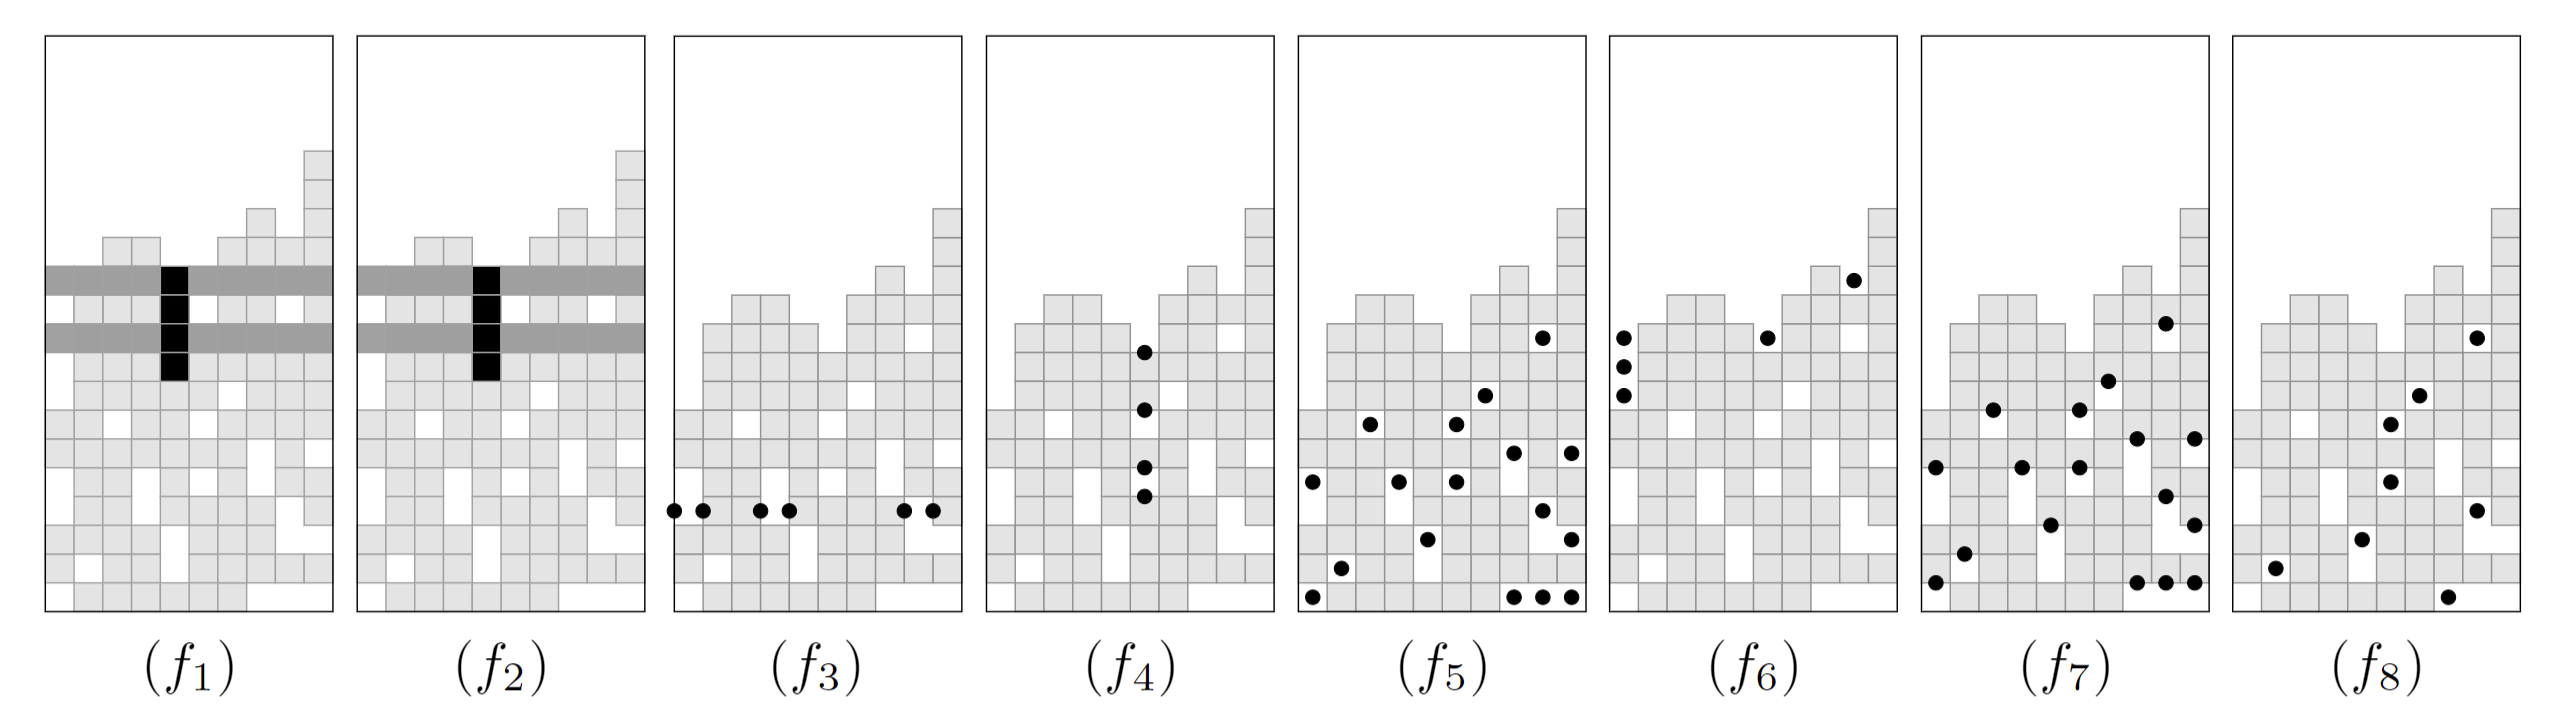
\includegraphics[width=0.8\linewidth]{features.png}
  \caption{Collection of parameters to describe Tetris state.}
\end{figure}

\begin{enumerate}
  \item $f_1$ (Landing Height): The height at which the current piece lands. In general, the lower a piece lands in Tetris, the better since the game ends when a piece goes too high.
  \item $f_2$ (Eroded Pieces): The number of cleared rows times the number of cells the current piece contributed to each of the cleared rows. This feature codifies how effective the placement of the current piece will be in terms of rows cleared: the end goal of the model.
  \item $f_3$ (Row Transitions): Including left and right borders as filled, the number of filled cells either to the right or left of an empty cell. In general it is preferable to have contiguous open space meaning the more filled cells to the left or right of a cleared cell, the worse.
  \item $f_4$ (Column Transitions): Including the bottom border as filled, the number of filled cells either to the below or above an empty cell. In general it is preferable to have contiguous open space meaning the more filled cells above or below a cleared cell, the worse.
  \item $f_5$ (Number of Holes): The number of cells with at least one filled cell above (and no clear cells directly above). Holes represent inefficiency in the stacking of pieces since the rows they are on cannot be cleared unless all the rows above are cleared.
  \item $f_6$ (Cumulative Wells): Defining a well as a local column-height minimum, the total number of cells in all wells. Wells make certain types of pieces hard to place. The easiest placement is on a flat surface (i.e., $f_6(s) = 0$).
  \item $f_7$ (Hole Depth): The total number of cells above all holes (as defined above). This enumerates the number of rows that need to be cleared to remove an inefficient hole.
  \item $f_8$ (Row Hole): The number of rows with holes. Any row with a hole represents inefficiency.
\end{enumerate}

\section{Approach}
\textbf{Clearly describe your approach and the algorithm you used. Note that you do not necessarily have to use RL to solve this problem (e.g. you can use a variant of the cross-entropy method.)}

To train our Tetris player, we used black box optimization via Cross-Entropy Method (CEM) to find the weights that would result in the best policy under the objective function laid out by [1].

To intelligently kickstart CEM and reduce training time, we intuited that the weights for all features but $f_2$ should be positive as they represent features we would like to avoid during play. $f_2$ represents an action which generates reward for our player, so we assumed it should be weighted negatively, reducing the cost of the action.

During each step of CEM, the weights are normalized to bound the parameter space we are exploring. 25 samples are taken under the gaussian distributions of our weights, with performance averaged over 25 games of Tetris. After computing the mean and variance of the elite performers, noise is added to the variance of our next set of gaussian distributions to reduce the liklihood of early convergence to a local optimum. The noise term decreases as iteration count increases according to an equation inspried by [2].

\[Z_t = \max(0.05, t/1000,0)\]

After iteration 50, the noise is clamped to 0, allowing our optimization to converge smoothly to a final, optimal solution.

Each game of Tetris can take a very long time to play through, especially once it is clearing 50,000 or more lines. When playing $625$ games per iteration, this means massive compute times to reach the point of convergence. To reduce training time, we implemented a technique proposed by literature [1] which introduces a bias to the random distribution of pieces. "Z" and "S" pieces are the most difficult to place as they often create holes in the wall. This causes the game to end faster, but has no adverse effects on training. If anything, the policy improves under this training distribution as it ends up being trained for a "worst-case scenario." As hundreds of thousands of turns go by, it is certain that periods of time will go by where "Z" and "S" pieces occur randomly many times in a row. To implement this training distribution, the TetrisEnv class was given the option of being instantiated in "training" mode. Under this mode, the $get\_random\_piece()$ method will return a "Z" or "S" piece with a 6/11 probability. Since this results in earlier game termination, the score obtained during optimization is not reflective of the final, evenly-distributed gameplay score.


\section{Evaluation}
Describe the performance of your agent, and make sure to include maximum and average lines cleared over 20 games.

During optimization, the performance of our Tetris AI quickly out-performed the 10,000 line threshold. After approximately 90 iterations of CEM, the method had firmly converged to a final set of weights (values are truncated to 6 decimal places to fit on one line)

\[w = \begin{bmatrix}
    0.340010 &
    0.045845 &
    0.406443 &
    0.452428 &
    0.429135 &
    0.067301 &
    0.127938 &
    0.554389 &
  \end{bmatrix}\]

\begin{figure}[h!]
  \centering
  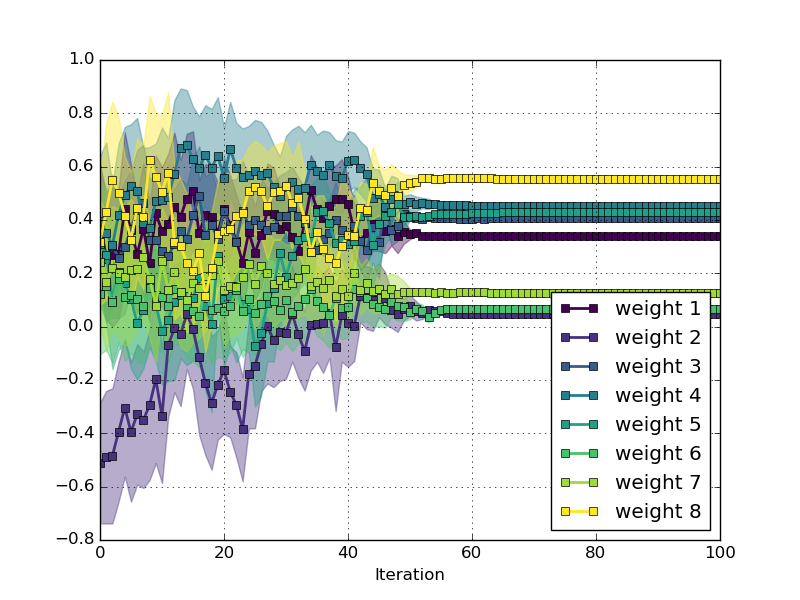
\includegraphics[width=0.7\linewidth]{weights.png}
  \caption{"Convergence of weights from 0 to 100 iterations of CEM."}
\end{figure}

\begin{figure}[h!]
  \centering
  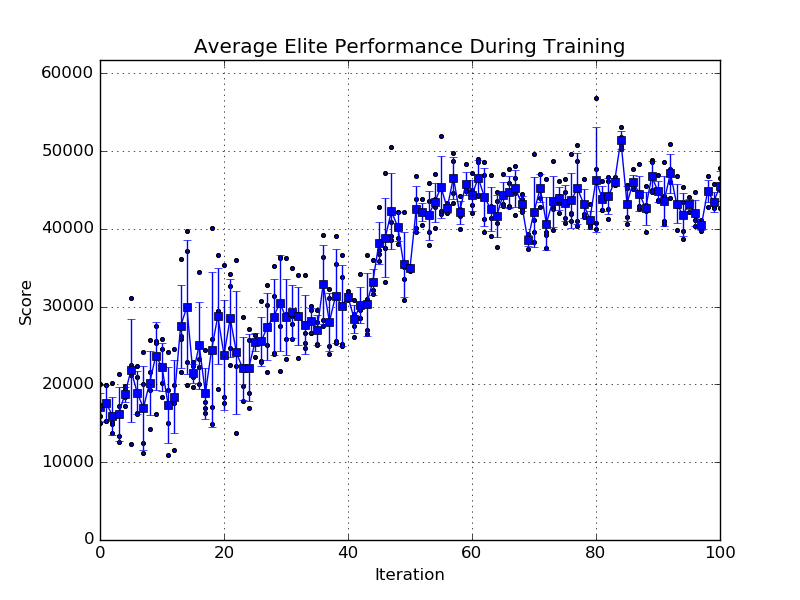
\includegraphics[width=0.7\linewidth]{training_scores.png}
  \caption{Scores of elites performers during training (lines cleared $\approx \text{score}/100$)}
\end{figure}

\begin{figure}[h!]
  \centering
  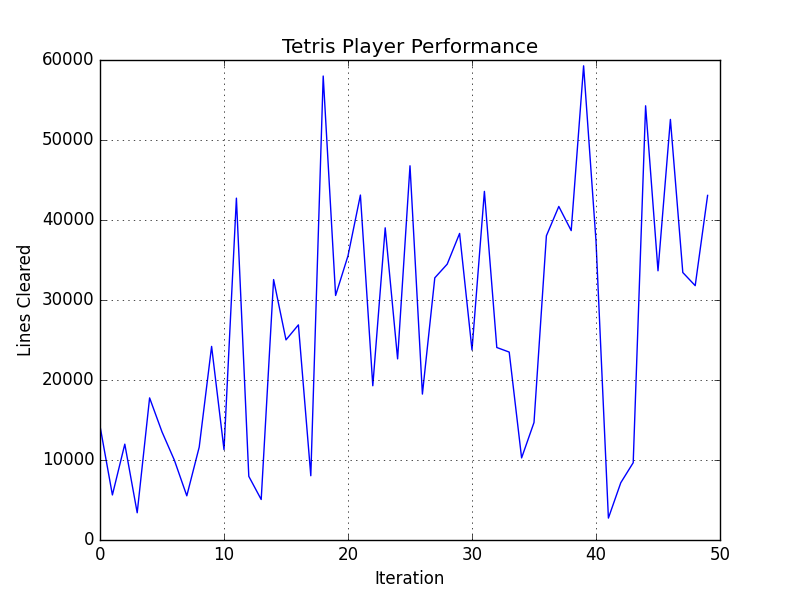
\includegraphics[width=0.7\linewidth]{performance.png}
  \caption{Scores of elites performers during training (lines cleared $\approx \text{score}/100$)}
\end{figure}

\section{References}

\begin{enumerate}[label={[\arabic*]}]
  \item B., Amine. “How to design good Tetris players.” HAL Open Science, https://hal.inria.fr/ hal-00926213/document, 2013

  \item I. Szita and A. Lörincz. “Learning tetris using the noisy cross-entropy method.” Neural Comput., 18(12):2936–2941, 2006.
\end{enumerate}


\end{document}
